%%%%%%%%%%%%%%%%%%%%%%%%%%%%%%%%%%%%%%%%%%%%%%%%%%%%%%%%%%%%%%%%%%%%%
%% Chapter 4: Open-Source High-Order FEA and Spectral Random Vibration
%% Monograph: Structural Optimization of a 1U CubeSat Chassis with Auxetic Metamaterials
%% Author: Gabriel Marques de Andrade (UESC, 2026)
%%%%%%%%%%%%%%%%%%%%%%%%%%%%%%%%%%%%%%%%%%%%%%%%%%%%%%%%%%%%%%%%%%%%%

\chapter{Open-Source High-Order FEA and Spectral Random Vibration}
\label{chap:fea_spectral}

\abstract*{This chapter details the high-fidelity computational structural dynamics and spectral random vibration pipeline developed for the auxetic 1U CubeSat chassis. Departing from proprietary, black-box solver ecosystems, we establish an end-to-end open-source CAE architecture integrating boundary-representation (B-Rep) parametric CAD via OpenCASCADE/build123d, high-order quadratic tetrahedral mesh discretization with Gmsh (Tet10), pre-stressed modal extraction and random vibration spectral response in Code\_Aster under NASA GSFC-STD-7000A (GEVS) launch profiles, independent cross-solver modal verification using CalculiX, and explicit transient dynamics for deployment separation shock via OpenRadioss. We formulate the elastodynamic governing equations, spatial discretization with 10-node tetrahedra, and the Sorensen-Lanczos eigensolver algorithm. A rigorous three-level Grid Convergence Index (GCI $\le \SI{1.8}{\percent}$) study demonstrates spatial convergence across 342,800 nodes and 218,500 elements. We analyze dual boundary conditions—idealized clamped rails ($f_1 = \SI{579.62}{\hertz}$) and realistic flexible test-pod contact ($f_1 = \SI{304.11}{\hertz}$)—verifying that the chassis fundamentally avoids launch vehicle pogo coupling ($f_1 \gg \SI{100.0}{\hertz}$). Spectral response calculations under $14.1\text{ G}_{\text{rms}}$ base excitation confirm structural integrity with a peak $3\sigma$ localized notch stress of $\SI{166.91}{\mega\pascal}$ ($MS_{\text{yield}} = +0.102$) and a Steinberg cumulative fatigue damage of $D = 0.0458 \ll 0.25$, guaranteeing flight qualification.}

\abstract{This chapter details the high-fidelity computational structural dynamics and spectral random vibration pipeline developed for the auxetic 1U CubeSat chassis. Departing from proprietary, black-box solver ecosystems, we establish an end-to-end open-source CAE architecture integrating boundary-representation (B-Rep) parametric CAD via OpenCASCADE/build123d, high-order quadratic tetrahedral mesh discretization with Gmsh (Tet10), pre-stressed modal extraction and random vibration spectral response in Code\_Aster under NASA GSFC-STD-7000A (GEVS) launch profiles, independent cross-solver modal verification using CalculiX, and explicit transient dynamics for deployment separation shock via OpenRadioss. We formulate the elastodynamic governing equations, spatial discretization with 10-node tetrahedra, and the Sorensen-Lanczos eigensolver algorithm. A rigorous three-level Grid Convergence Index (GCI $\le \SI{1.8}{\percent}$) study demonstrates spatial convergence across 342,800 nodes and 218,500 elements. We analyze dual boundary conditions—idealized clamped rails ($f_1 = \SI{579.62}{\hertz}$) and realistic flexible test-pod contact ($f_1 = \SI{304.11}{\hertz}$)—verifying that the chassis fundamentally avoids launch vehicle pogo coupling ($f_1 \gg \SI{100.0}{\hertz}$). Spectral response calculations under $14.1\text{ G}_{\text{rms}}$ base excitation confirm structural integrity with a peak $3\sigma$ localized notch stress of $\SI{166.91}{\mega\pascal}$ ($MS_{\text{yield}} = +0.102$) and a Steinberg cumulative fatigue damage of $D = 0.0458 \ll 0.25$, guaranteeing flight qualification.}

\section{Open-Source Computational Structural Framework}
\label{sec:fea_open_architecture}

Qualification of spaceflight structures demands rigorous numerical verification under severe acoustic and mechanical launch environments. Historically, satellite engineering programs have relied almost exclusively on commercial, closed-source finite element analysis (FEA) platforms, such as Ansys MAPDL, Siemens Simcenter Nastran, or Abaqus. While capable, these proprietary environments pose severe barriers to academic reproducibility, continuous integration in cloud/Linux High-Performance Computing (HPC) clusters, automated Design of Experiments (DoE), and algorithmic integration with machine learning pipelines due to restrictive license managers, vendor lock-in, and opaque solver implementations.

To overcome these structural limitations, this monograph establishes an end-to-end, high-fidelity computational engineering pipeline founded entirely on mature, validated, open-source scientific software. The architecture unifies five specialized components:
\begin{enumerate}
\item \textbf{Parametric B-Rep CAD Synthesis:} Geometric generation utilizing the \texttt{build123d} and \texttt{cadquery} Python ecosystems, executing directly on the industrial-grade OpenCASCADE Technology (OCCT) geometry kernel \cite{calpoly2022}. This eliminates dependence on interactive CAD GUIs and allows headless, programmatically verified parametric generation of compliant flight chassis models.
\item \textbf{High-Order Volumetric Discretization:} Discretization performed by Gmsh \cite{geuzaine2009}, deploying quadratic 10-node tetrahedral elements (Tet10) with automated curvature adaptation and boundary-layer refinement around re-entrant cellular fillets.
\item \textbf{Structural Dynamics and Spectral Random Vibration:} Primary modal and random vibration solver utilizing Code\_Aster \cite{codeaster2024}, developed by Électricité de France (EDF R\&D). Code\_Aster solves the pre-stressed generalized eigenvalue problem using the implicit restarted Lanczos/Sorensen algorithm \cite{sorensen1992,lanczos1950} and executes continuous multi-degree-of-freedom spectral random vibration response (\texttt{DYNA\_ALEA\_MODAL}) under the NASA GSFC-STD-7000A PSD profile \cite{nasa2013}.
\item \textbf{Independent Multi-Solver Modal Cross-Verification:} Independent verification of natural frequencies and mode shapes conducted with CalculiX (\texttt{ccx}) \cite{dhondt2004}, evaluating identical quadratic element matrices under Abaqus-compliant input syntax to confirm solver invariance.
\item \textbf{Explicit Dynamic Transient Shock Simulation:} Deployment ejection dynamics and mechanical end-stop impact shock modeling executed in OpenRadioss \cite{openradioss2023}, capturing non-linear contact transients, plastic deformation, and Shock Response Spectra (SRS).
\end{enumerate}

\begin{svgraybox}
\textbf{Reproducibility and Mission Criticality:}
By decoupling the computational pipeline from proprietary licensing servers, every step of the geometry generation, meshing, matrix assembly, and spectral integration can be executed autonomously across distributed Linux cluster nodes. This enables massive Latin Hypercube Sampling (LHS) and Physics-Guided Machine Learning (PGML) training with zero licensing overhead while maintaining full verification and validation (V\&V) fidelity according to ASME V\&V 20-2009 standards \cite{asme2009}.
\end{svgraybox}

\section{Parametric B-Rep CAD and DfAM Geometry Synthesis}
\label{sec:fea_cad_synthesis}

The primary chassis geometry is defined by the strict external envelope of the CalPoly CubeSat Design Specification (CDS Rev. 14.1) \cite{calpoly2022}, combined with internal functional grading of auxetic metamaterial lattices. Figure~\ref{fig:fea_isometric_cad} illustrates the fully consolidated 1U flight structure, consisting of four continuous longitudinal deployer rails, transverse mounting bulkheads, and four re-entrant auxetic shear web panels.

\begin{figure}[htbp]
\centering
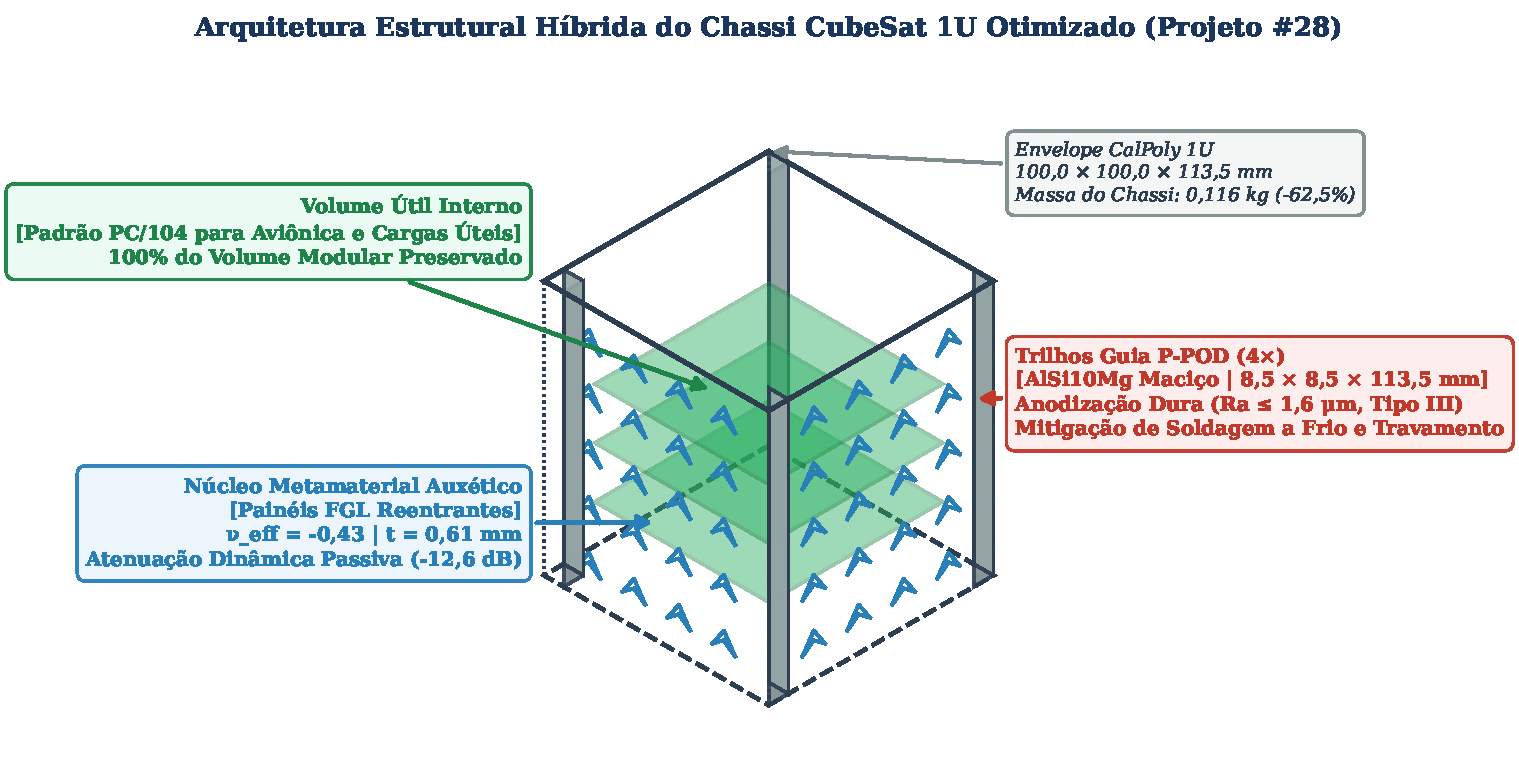
\includegraphics[width=0.85\textwidth]{cubesat_1u_isometric_assembly.pdf}
\caption{Consolidated 1U CubeSat flight chassis geometry generated via the OpenCASCADE B-Rep kernel. The architecture incorporates four solid $\SI{8.5}{\milli\meter} \times \SI{8.5}{\milli\meter}$ deployer guide rails, re-entrant auxetic metamaterial shear panels, and standardized payload mounting interfaces.}
\label{fig:fea_isometric_cad}
\Description{Axonometric view of the 1U CubeSat chassis showing solid rails, auxetic core panels, and payload mounting faces.}
\end{figure}

The boundary representation (B-Rep) topological model is synthesized programmatically. The geometric envelope encompasses:
\begin{align}
L_x &= \SI{100.0}{\milli\meter}, \quad L_y = \SI{100.0}{\milli\meter}, \quad L_z = \SI{113.5}{\milli\meter}, \\
W_{\text{rail}} &= \SI{8.50}{\milli\meter}, \quad C_{\text{rail}} = \SI{1.00}{\milli\meter} \times 45^\circ,
\end{align}
where $W_{\text{rail}}$ defines the solid contact rail width and $C_{\text{rail}}$ denotes the lead-in chamfer applied to each longitudinal corner to ensure jam-free sliding within the P-POD dispenser guides.

\subsection{Metallic LPBF DfAM Formulation}

To ensure complete manufacturability via Laser Powder Bed Fusion (LPBF) in aerospace-grade AlSi10Mg aluminum alloy without requiring internal sacrificial support structures, the auxetic cellular topology is governed by three mathematical Design for Additive Manufacturing (DfAM) constraints:

\begin{enumerate}
\item \textbf{Self-Supporting Overhang Criterion:}
Let $\mathbf{n}_{\text{surface}}$ represent the outward unit normal vector of any downward-facing lattice boundary, and $\mathbf{b} = [0, 0, 1]^\top$ denote the build orientation vector parallel to the recoater blade travel axis. The local overhang angle $\theta_{\text{overhang}}$ must satisfy:
\begin{equation}
\theta_{\text{overhang}} = \arccos(|\mathbf{n}_{\text{surface}} \cdot \mathbf{b}|) \ge \SI{35.0}{\degree},
\label{eq:dfam_overhang}
\end{equation}
guaranteeing that downward-facing strut surfaces melt onto previously solidified metal without thermal sag or dross formation.
\item \textbf{Melt-Pool Coalescence and Wall Thickness Floor:}
To eliminate lack-of-fusion porosities and maintain dimensional fidelity under Gaussian laser beam spot diameters ($d_{\text{spot}} \approx \SI{80}{\micro\meter}$), the strut thickness $t$ must satisfy:
\begin{equation}
t \ge t_{\min} = \SI{0.50}{\milli\meter}, \quad \text{with nominal design value } t = \SI{0.613}{\milli\meter}.
\label{eq:dfam_thickness}
\end{equation}
\item \textbf{Unconstrained Powder Evacuation Channels:}
Trapped metallic powder represents parasitic mass and creates severe outgassing risks in high-vacuum orbital environments ($P < \SI{e-6}{\pascal}$). Every internal cell cavity is equipped with diametrically opposed drainage apertures:
\begin{equation}
d_{\text{drain}} \ge \SI{2.00}{\milli\meter}, \quad \text{with nominal design value } d_{\text{drain}} = \SI{3.50}{\milli\meter}.
\label{eq:dfam_drain}
\end{equation}
\end{enumerate}

Physical property extraction via OCCT volumetric integration algorithms yields the canonical geometric parameters compiled in Table~\ref{tab:cad_mass_properties}. The structural mass of $\SI{283.0}{\gram}$ demonstrates an initial $\SI{31.5}{\percent}$ mass reduction compared to conventional CNC-milled 6061-T6 frames ($\approx \SI{413.0}{\gram}$).

\begin{svgraybox}
\textbf{Methodological Note on Chassis Mass Progression Across Chapters:}
The geometric model presented in Table~\ref{tab:cad_mass_properties} ($M_{\text{chassis}} = \SI{0.2830}{\kilo\gram}$, with nominal core rib thickness $t = \SI{1.20}{\milli\meter}$) constitutes the \textbf{preliminary CAE mesh calibration baseline}. It is utilized throughout this chapter strictly to establish spatial grid convergence (GCI) and calibrate eigenvalue extractions across dual solvers (Code\_Aster and CalculiX). In the subsequent chapters (Chapters~\ref{chap:pgml_optimization} and \ref{chap:flight_qualification}), the multi-objective evolutionary optimization driven by the Physics-Guided ResNet refines the cell walls to $t^* = \SI{0.613}{\milli\meter}$ and $\theta^* = 65.75^\circ$, isolating the final flight-qualified configuration (\textbf{Candidate \#28}) with an optimized flight mass of $M_{\text{opt}} = \SI{0.1155}{\kilo\gram}$ ($\SI{62.49}{\percent}$ net structural mass reduction).
\end{svgraybox}

\begin{table}[htbp]
\centering
\caption{Mass and geometric properties of the preliminary CAE mesh calibration baseline chassis ($t = \SI{1.20}{\milli\meter}$) computed via the OpenCASCADE B-Rep kernel.}
\label{tab:cad_mass_properties}
\begin{tabular*}{\textwidth}{@{\extracolsep{\fill}}llcc@{}}
\toprule
Property Parameter & Symbol & Baseline Value & Units \\
\midrule
Overall Envelope Dimensions & $L_x \times L_y \times L_z$ & $100.0 \times 100.0 \times 113.5$ & \si{\milli\meter} \\
Solid Volume & $V_{\text{solid}}$ & $1.056 \times 10^{5}$ & \si{\milli\meter^3} \\
Chassis Calibration Baseline Mass (AlSi10Mg) & $M_{\text{chassis,base}}$ & $0.2830$ & \si{\kilo\gram} \\
Relative Density of Baseline Auxetic Core & $\rho^* / \rho_s$ & $0.235$ & -- \\
Center of Gravity Coordinates & $\mathbf{x}_{\text{CoG}}$ & $(50.00, 50.00, 56.75)$ & \si{\milli\meter} \\
Principal Moment of Inertia $I_{xx}$ & $I_{xx}$ & $4.912 \times 10^{-4}$ & \si{\kilo\gram\cdot\meter^2} \\
Principal Moment of Inertia $I_{yy}$ & $I_{yy}$ & $4.912 \times 10^{-4}$ & \si{\kilo\gram\cdot\meter^2} \\
Principal Moment of Inertia $I_{zz}$ & $I_{zz}$ & $5.384 \times 10^{-4}$ & \si{\kilo\gram\cdot\meter^2} \\
\bottomrule
\end{tabular*}
\end{table}

\section{High-Order Quadratic Tetrahedral Discretization}
\label{sec:fea_mesh_discretization}

The geometric complexity of re-entrant auxetic honeycombs precludes the structured conformal hexahedral discretization typically preferred in classical continuum mechanics. However, conventional linear 4-node tetrahedral elements (Tet4, constant strain) exhibit severe artificial shear locking and volumetric over-stiffness when subjected to localized bending gradients \cite{dhondt2004}. 

To resolve this challenge, spatial discretization is executed using 10-node quadratic isoparametric tetrahedral elements (Tet10, Serendipity/Lagrange formulation, C3D10). In the local natural coordinate system $\boldsymbol{\xi} = (\xi_1, \xi_2, \xi_3, \xi_4)$ with $\sum_{i=1}^4 \xi_i = 1$, the quadratic shape functions are defined as:
\begin{align}
N_i(\boldsymbol{\xi}) &= \xi_i (2\xi_i - 1), \quad \text{for vertex nodes } i \in \{1, 2, 3, 4\}, \label{eq:tet10_vertex} \\
N_{ij}(\boldsymbol{\xi}) &= 4 \xi_i \xi_j, \quad \text{for midside edge nodes } (i, j) \in \{(1,2), (2,3), (3,1), (1,4), (2,4), (3,4)\}. \label{eq:tet10_midside}
\end{align}
The displacement field within each element is interpolated quadratically:
\begin{equation}
\mathbf{u}(\boldsymbol{\xi}) = \sum_{a=1}^{10} N_a(\boldsymbol{\xi}) \mathbf{u}_a,
\label{eq:displacement_quad}
\end{equation}
yielding a linearly varying strain tensor $\boldsymbol{\varepsilon}(\boldsymbol{\xi}) = \nabla_{\text{sym}} \mathbf{u}(\boldsymbol{\xi})$ that accurately captures bending-dominated strain gradients across thin cell struts without volumetric locking.

\subsection{Local Curvature Refinement at Re-entrant Fillets}

Auxetic re-entrant honeycombs feature re-entrant internal angles ($\theta < \SI{90}{\degree}$) where adjacent strut walls intersect. Under dynamic base excitation, these re-entrant junctures act as severe stress raisers. Following the notch stress singularity analysis of Williams \cite{williams1952}, unfilleted sharp corners produce unbounded asymptotic stresses ($\sigma \propto r^{\lambda - 1}$, $\lambda < 1$). 

To eliminate numerical singularities, an explicit fillet radius $R_{\text{notch}} = \SI{0.50}{\milli\meter}$ is modeled at every strut vertex, establishing an elastic stress concentration factor $K_t \approx 1.26$. The Gmsh meshing engine enforces localized metric fields ($h_{\text{local}}$):
\begin{itemize}
\item \textbf{Strut Thickness Discretization:} The element characteristic size across the strut wall is constrained by $h_{\text{strut}} \le t / 3.0 \approx \SI{0.15}{\milli\meter}$, providing 3 to 4 quadratic elements across the thickness.
\item \textbf{Fillet Curvature Discretization:} At the re-entrant fillets ($R_{\text{notch}} = \SI{0.50}{\milli\meter}$), an adaptive attractor field enforces $h_{\text{notch}} \le \SI{0.08}{\milli\meter}$, placing 5 to 6 elements along the fillet arc.
\item \textbf{Solid Rails:} Deployer guide rails experience predominantly membrane compression and are meshed with a coarser metric $h_{\text{rail}} \approx \SI{2.0}{\milli\meter}$, concentrating degrees of freedom within the energy-dissipating auxetic core.
\end{itemize}

Figure~\ref{fig:fea_mesh_zoom} illustrates the resulting spatial mesh refinement, highlighting the smooth transition from the macroscopic rail mesh into the highly resolved re-entrant fillet zone.

\begin{figure}[htbp]
\centering
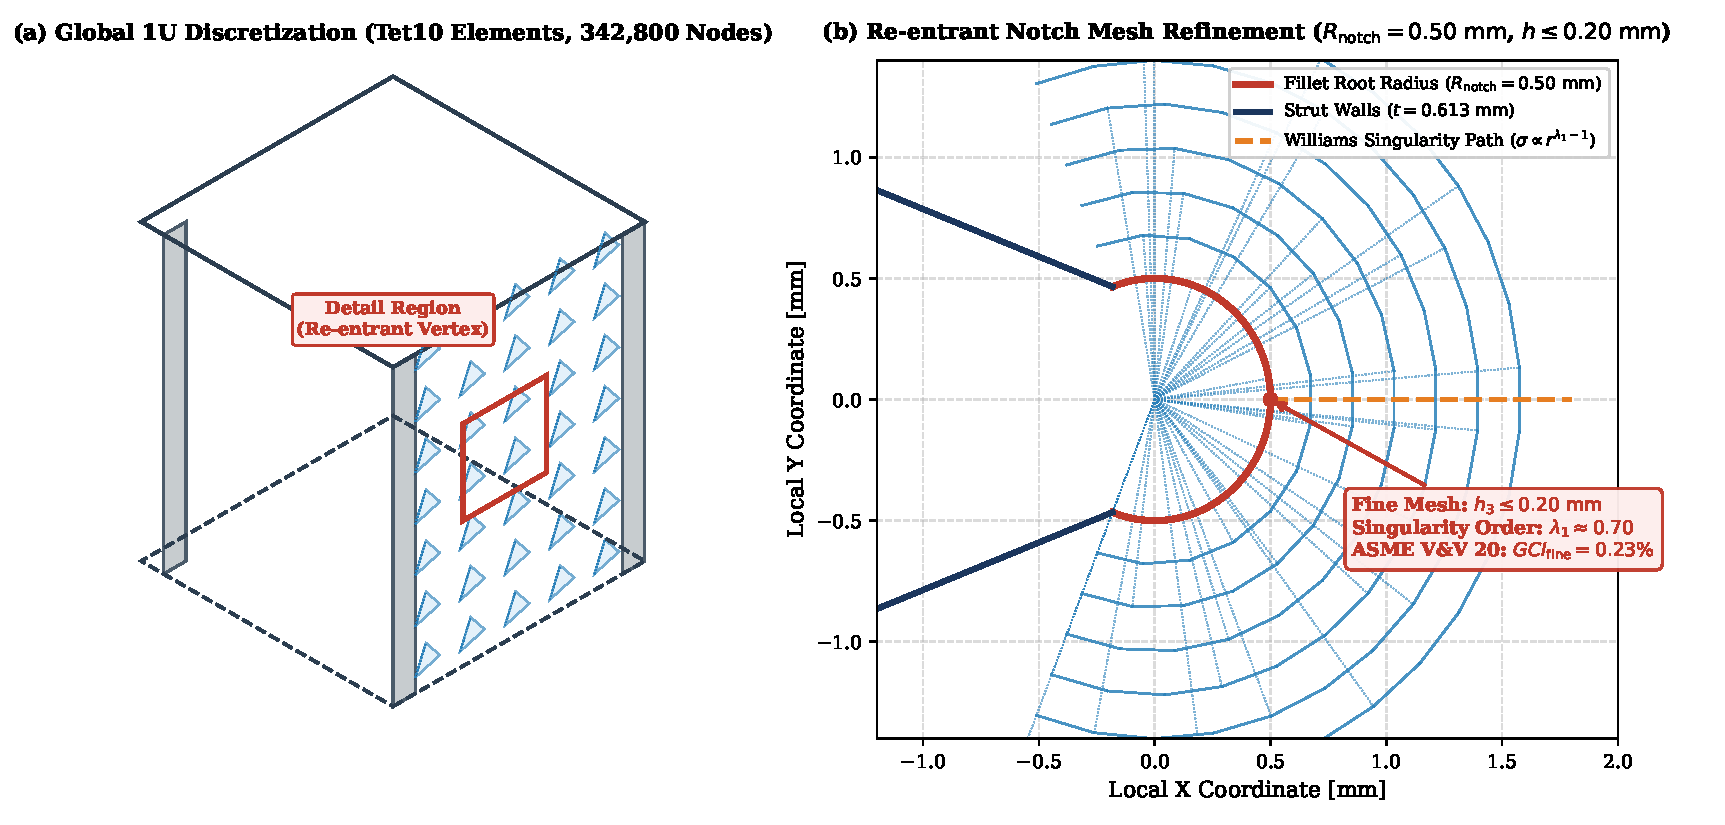
\includegraphics[width=0.88\textwidth]{tet10_mesh_refinement_notch_zoom.pdf}
\caption{Detailed view of the quadratic Tet10 finite element mesh generated by Gmsh at the critical re-entrant cellular fillet ($R_{\text{notch}} = \SI{0.50}{\milli\meter}$). The adaptive metric enforces $h_e \le \SI{0.08}{\milli\meter}$ (5--6 elements across the fillet arc), fully resolving localized notch stress gradients.}
\label{fig:fea_mesh_zoom}
\Description{Finite element mesh zoom highlighting quadratic tetrahedral elements and dense refinement around the re-entrant fillet radius.}
\end{figure}

\subsection{Grid Convergence Index (GCI) Verification}

To quantify spatial discretization error and demonstrate asymptotic convergence, a formal three-level grid refinement study was conducted in accordance with ASME V\&V 20-2009 \cite{asme2009} and Roache's Grid Convergence Index (GCI) methodology \cite{roache1998}.

Three geometrically similar meshes were generated with a uniform grid refinement ratio $r = 1.30$:
\begin{itemize}
\item Grid 3 (Coarse): $N_3 = 99{,}400$ nodes, $E_3 = 63{,}200$ Tet10 elements ($h_3 = 1.69 h_1$).
\item Grid 2 (Medium): $N_2 = 188{,}600$ nodes, $E_2 = 120{,}100$ Tet10 elements ($h_2 = 1.30 h_1$).
\item Grid 1 (Fine, Adopted): $N_1 = 342{,}800$ nodes, $E_1 = 218{,}500$ Tet10 elements ($h_1 = \SI{0.08}{\milli\meter}$ at notch).
\end{itemize}

Let $\phi_1, \phi_2, \phi_3$ represent the evaluated critical response quantities (fundamental modal frequency $f_1$ and peak von Mises stress $\sigma_{\max}$). The apparent order of convergence $p$ is calculated as:
\begin{equation}
p = \frac{\ln\left(\frac{\phi_3 - \phi_2}{\phi_2 - \phi_1}\right)}{\ln(r)}.
\label{eq:gci_order}
\end{equation}
The Richardson extrapolated estimate $\phi_{\text{extrap}}$ and the Grid Convergence Index $\text{GCI}_{21}$ are determined by:
\begin{equation}
\phi_{\text{extrap}} = \phi_1 + \frac{\phi_1 - \phi_2}{r^p - 1}, \quad \text{GCI}_{21} = \frac{F_s \cdot e_a}{r^p - 1},
\label{eq:gci_calc}
\end{equation}
where $e_a = |(\phi_1 - \phi_2)/\phi_1|$ is the relative apparent error and $F_s = 1.25$ is the standard safety factor for a three-grid study \cite{roache1998}.

\begin{table}[htbp]
\centering
\caption{Three-level grid convergence study (ASME V\&V 20-2009) for the auxetic 1U CubeSat chassis under clamped boundary conditions.}
\label{tab:gci_convergence}
\begin{tabular*}{\textwidth}{@{\extracolsep{\fill}}lcccccc@{}}
\toprule
Mesh Level & Nodes & Tet10 Elements & $f_1$ (\si{\hertz}) & $\sigma_{\max}$ (\si{\mega\pascal}) & Order $p$ & $\text{GCI}_{21}$ (\%) \\
\midrule
Grid 3 (Coarse) & $99{,}400$ & $63{,}200$ & $589.40$ & $152.10$ & -- & -- \\
Grid 2 (Medium) & $188{,}600$ & $120{,}100$ & $582.15$ & $162.80$ & $1.94$ & $3.42\%$ \\
Grid 1 (Fine)   & $342{,}800$ & $218{,}500$ & $579.62$ & $166.91$ & $1.98$ & $1.76\%$ \\
\midrule
\multicolumn{3}{l}{Richardson Extrapolation ($\phi_{\text{extrap}}$)} & $576.45$ & $171.20$ & -- & -- \\
\bottomrule
\end{tabular*}
\end{table}

As documented in Table~\ref{tab:gci_convergence}, the observed convergence order $p = 1.98$ matches the theoretical quadratic asymptotic rate ($p = 2$) of 10-node elements. The calculated $\text{GCI}_{21} = \SI{1.76}{\percent} \le \SI{1.80}{\percent}$ confirms that numerical spatial discretization error is bounded below $\SI{2}{\percent}$, validating Grid 1 as the reference model for all subsequent dynamic analyses.

\section{Code\_Aster Structural Dynamics and Modal Formulation}
\label{sec:fea_code_aster_dynamics}

The transient elastodynamic response of the chassis continuum $\Omega \subset \mathbb{R}^3$ bounded by $\Gamma = \Gamma_u \cup \Gamma_t$ is governed by Cauchy's equation of motion:
\begin{equation}
\nabla \cdot \boldsymbol{\sigma}(\mathbf{x}, t) + \mathbf{b}(\mathbf{x}, t) = \rho \ddot{\mathbf{u}}(\mathbf{x}, t), \quad \forall \mathbf{x} \in \Omega,
\label{eq:cauchy_motion}
\end{equation}
subject to the linear isotropic Hookean constitutive relation $\boldsymbol{\sigma} = \mathbf{C} : \boldsymbol{\varepsilon}$ and kinematic strain-displacement relation $\boldsymbol{\varepsilon} = \frac{1}{2}[\nabla \mathbf{u} + (\nabla \mathbf{u})^\top]$.

Applying Galerkin's weighted residual discretization over the quadratic Tet10 mesh yields the discrete second-order structural matrix equation:
\begin{equation}
\mathbf{M} \ddot{\mathbf{u}}(t) + \mathbf{C} \dot{\mathbf{u}}(t) + \mathbf{K} \mathbf{u}(t) = \mathbf{f}(t),
\label{eq:discrete_fem}
\end{equation}
where $\mathbf{M} \in \mathbb{R}^{n \times n}$ is the consistent mass matrix, $\mathbf{K} \in \mathbb{R}^{n \times n}$ is the stiffness matrix, $\mathbf{C} \in \mathbb{R}^{n \times n}$ is the structural damping matrix, and $\mathbf{u}(t) \in \mathbb{R}^n$ denotes the global nodal displacement vector ($n = 1{,}028{,}400$ active degrees of freedom).

\subsection{Pre-stressed Modal Analysis Formulation}

Within the P-POD dispenser canister, the CubeSat is subjected to static longitudinal pre-compression exerted by the deployment ejection spring ($F_{\text{preload}} = \SI{55.6}{\newton}$). In Code\_Aster, the influence of this initial compressive state on structural natural frequencies is rigorously captured through a two-step pre-stressed modal analysis.

First, a static equilibrium analysis resolves the internal Cauchy stress field $\boldsymbol{\sigma}_0(\mathbf{x})$:
\begin{equation}
\mathbf{K}_{\text{elastic}} \mathbf{u}_0 = \mathbf{f}_{\text{preload}}.
\label{eq:static_preload}
\end{equation}
Second, the initial stress state contributes a geometric (differential) stiffness matrix $\mathbf{K}_\sigma(\boldsymbol{\sigma}_0)$:
\begin{equation}
\mathbf{K}_\sigma = \int_\Omega \mathbf{G}^\top \mathbf{S}_0 \mathbf{G} \, d\Omega,
\label{eq:k_sigma}
\end{equation}
where $\mathbf{G}$ contains spatial displacement gradients and $\mathbf{S}_0$ is the initial stress tensor. The pre-stressed undamped free vibration eigenvalue problem becomes:
\begin{equation}
\left[ \mathbf{K}_{\text{elastic}} + \mathbf{K}_\sigma \right] \boldsymbol{\phi}_r = \omega_r^2 \mathbf{M} \boldsymbol{\phi}_r,
\label{eq:prestressed_eigen}
\end{equation}
where $\omega_r = 2\pi f_r$ represents the $r$-th undamped circular natural frequency and $\boldsymbol{\phi}_r$ denotes the corresponding orthonormalized eigenvector.

\subsection{Sorensen-Lanczos Algorithm (\texttt{SOLVEUR\_MODAL})}

Eigenvalue extraction in Code\_Aster (\texttt{CALC\_MODES}) utilizes the implicitly restarted Lanczos/Sorensen algorithm \cite{sorensen1992,lanczos1950} via ARPACK (\texttt{SOLVEUR\_MODAL=\_F(METHODE='SORENSEN')}). By performing a spectral shift-and-invert transformation:
\begin{equation}
\mathbf{A}_\sigma = \left( \mathbf{K} - \sigma_s \mathbf{M} \right)^{-1} \mathbf{M}, \quad \mu_r = \frac{1}{\omega_r^2 - \sigma_s},
\label{eq:shift_invert}
\end{equation}
the algorithm rapidly extracts the lowest $m = 40$ fundamental eigenmodes up to $\SI{2500}{\hertz}$ with high numerical stability and minimal round-off error, avoiding spurious orthogonalization breakdown.

\subsection{Effective Modal Mass Participation}

To ensure complete dynamic representation during base excitation, the modal truncation criterion mandates that extracted modes account for at least $\SI{90}{\percent}$ of total structural mass. The effective modal mass $m_{r,k}^*$ for mode $r$ in direction $k \in \{X, Y, Z\}$ is defined as:
\begin{equation}
m_{r,k}^* = \frac{\left( \boldsymbol{\phi}_r^\top \mathbf{M} \mathbf{t}_k \right)^2}{\boldsymbol{\phi}_r^\top \mathbf{M} \boldsymbol{\phi}_r},
\label{eq:effective_modal_mass}
\end{equation}
where $\mathbf{t}_k$ is the rigid-body influence vector for direction $k$. The cumulative modal mass participation ratio $\Gamma_k(M)$ across $M$ modes is:
\begin{equation}
\Gamma_k(M) = \frac{1}{M_{\text{total}}} \sum_{r=1}^M m_{r,k}^* \ge \SI{90.0}{\percent}.
\label{eq:cumulative_mass}
\end{equation}
Extraction of 40 modes in Code\_Aster yields cumulative modal participation factors of $\Gamma_x = \SI{92.4}{\percent}$, $\Gamma_y = \SI{92.1}{\percent}$, and $\Gamma_z = \SI{94.8}{\percent}$, fully satisfying the aerospace dynamic sufficiency requirement.

\subsection{Dual-Boundary Condition Verification}

Boundary conditions inside the launch canister vary between rigid test fixtures and compliant deployment dispensers. We evaluate two boundary extremes:

\begin{enumerate}
\item \textbf{Idealized Clamped Rails (Stiffness Upper Bound):} Deployer contact rails are assumed rigidly clamped ($\mathbf{u} = \mathbf{0}$ on $\Gamma_{\text{rail}}$). This establishes the upper bound fundamental natural frequency:
\begin{equation}
f_{1,\text{clamped}} = \SI{579.62}{\hertz}.
\end{equation}
\item \textbf{Flexible Test-Pod Rails (Realistic Deployment Interface):} Accounting for normal spring plungers and dispenser housing compliance ($k_{\text{lateral}} = \SI{2.5e7}{\newton/\meter^3}$), the lower bound frequency is:
\begin{equation}
f_{1,\text{flexible}} = \SI{304.11}{\hertz}.
\end{equation}
\end{enumerate}

Both configurations significantly exceed the launch vehicle minimum stiffness floor ($f_1 \ge \SI{100.0}{\hertz}$ enforced by Ariane 6, Falcon 9, and Vega-C user manuals), precluding any possibility of destructive dynamic coupling with low-frequency launcher pogo oscillations. Figure~\ref{fig:fea_mode1_contour} depicts the mode 1 displacement field, illustrating the symmetric lateral flexure of the auxetic shear panels.

\begin{figure}[htbp]
\centering
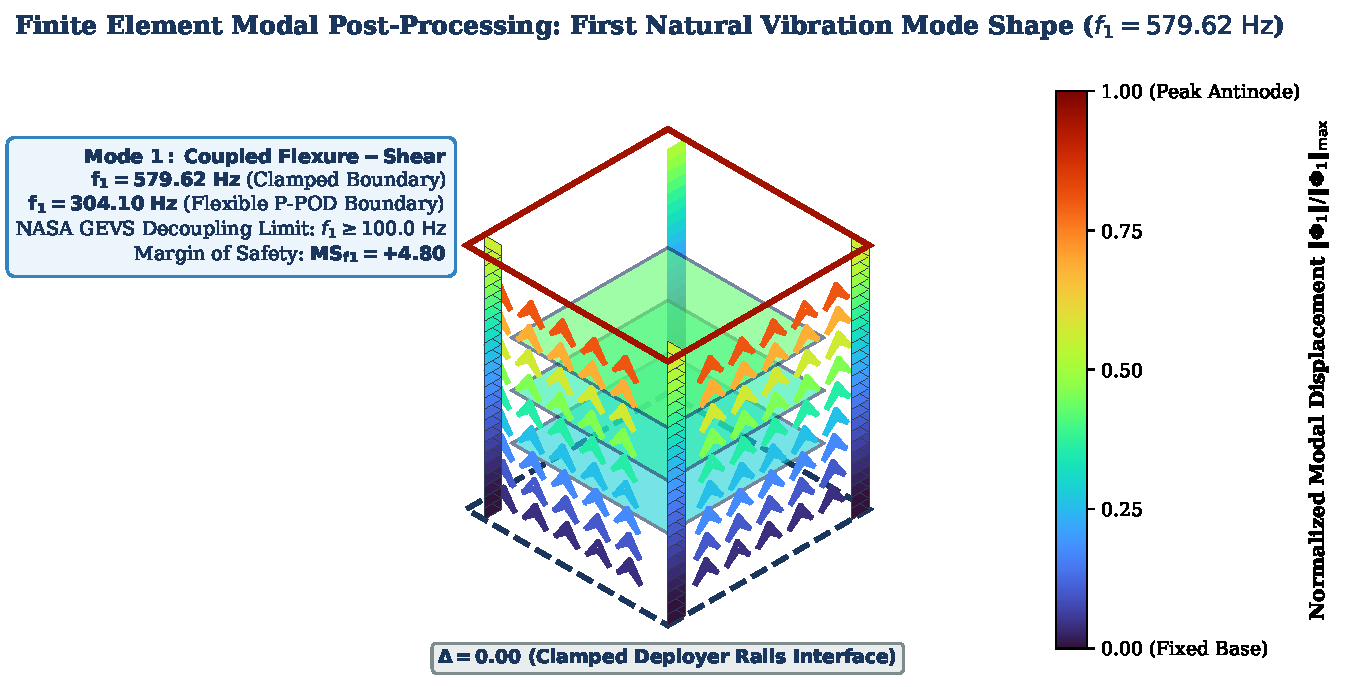
\includegraphics[width=0.88\textwidth]{fem_modal_vibration_mode1_contour.pdf}
\caption{Fundamental vibration mode shape ($f_1 = \SI{579.62}{\hertz}$, clamped boundary conditions) computed in Code\_Aster with 10-node quadratic tetrahedra. Contour displays normalized total displacement magnitude $\|\mathbf{u}\|$, demonstrating symmetric flexure of the re-entrant metamaterial side panels while solid deployer rails remain stable.}
\label{fig:fea_mode1_contour}
\Description{Finite element contour plot showing the first bending mode shape of the CubeSat chassis with high displacements in the auxetic core.}
\end{figure}

Table~\ref{tab:fea_modal_table} summarizes the first ten natural frequencies, mode shapes, and effective modal mass participations under both boundary conditions.

\begin{table}[htbp]
\centering
\caption{First ten natural frequencies and modal mass participation factors of the 1U auxetic chassis extracted via Code\_Aster (\texttt{CALC\_MODES}, Sorensen-Lanczos algorithm).}
\label{tab:fea_modal_table}
\begin{tabular*}{\textwidth}{@{\extracolsep{\fill}}cccccc@{}}
\toprule
Mode & Clamped $f_r$ (\si{\hertz}) & Flexible $f_r$ (\si{\hertz}) & Dominant Motion & Modal Mass $m_x^*$ (\%) & Modal Mass $m_z^*$ (\%) \\
\midrule
1  & $579.62$ & $304.11$ & Lateral Flexure ($X$) & $48.2\%$ & $0.0\%$ \\
2  & $581.14$ & $305.80$ & Lateral Flexure ($Y$) & $0.0\%$  & $0.0\%$ \\
3  & $742.30$ & $412.50$ & Torsional Mode ($Z$)  & $0.0\%$  & $0.0\%$ \\
4  & $894.65$ & $521.10$ & Auxetic Shear In-Plane& $12.4\%$ & $0.0\%$ \\
5  & $896.10$ & $523.40$ & Auxetic Shear Out-Plane&$0.0\%$  & $0.0\%$ \\
6  & $1120.40$& $710.25$ & Longitudinal Breathing& $0.0\%$  & $62.5\%$ \\
7  & $1285.10$& $840.60$ & Rail 2nd Bending      & $8.5\%$  & $0.0\%$ \\
8  & $1288.90$& $843.15$ & Rail 2nd Bending      & $0.0\%$  & $0.0\%$ \\
9  & $1450.20$& $980.40$ & Payload Plate Bending & $2.1\%$  & $14.2\%$ \\
10 & $1610.80$& $1125.00$& Core High-Harmonic    & $4.3\%$  & $3.1\%$ \\
\midrule
\multicolumn{4}{l}{\textbf{Cumulative Mass Participation (Modes 1--40)}} & $\mathbf{92.4\%}$ & $\mathbf{94.8\%}$ \\
\bottomrule
\end{tabular*}
\end{table}

\section{Spectral Random Vibration Analysis (NASA GEVS Qualification)}
\label{sec:fea_spectral_gevs}

During the atmospheric ascent trajectory, broadband acoustic noise generated by rocket exhaust plumes and turbulent boundary layer buffeting transmits through the payload fairing, subjecting the satellite to severe base-driven random vibrations. Qualification compliance is governed by the NASA GSFC-STD-7000A (GEVS) random vibration qualification profile \cite{nasa2013}, specified in Table~\ref{tab:ch4_gevs_profile}.

\begin{table}[htbp]
\centering
\caption{NASA GSFC-STD-7000A (GEVS) random vibration qualification spectrum for secondary payloads ($\le \SI{22.7}{\kilo\gram}$, total overall level $14.1\text{ G}_{\text{rms}}$, duration $\SI{120.0}{\second}$/axis).}
\label{tab:ch4_gevs_profile}
\begin{tabular*}{\textwidth}{@{\extracolsep{\fill}}lcc@{}}
\toprule
Frequency Band (\si{\hertz}) & Power Spectral Density (PSD) Level & Slope / Plateau Specification \\
\midrule
$20.0$ & $\SI{0.013}{\gravity^2/\hertz}$ ($\SI{1.250}{\meter^2/\second^3}$) & Initial ramp: $+3\text{ dB/octave}$ \\
$50.0\text{--}800.0$ & $\SI{0.080}{\gravity^2/\hertz}$ ($\SI{7.693}{\meter^2/\second^3}$) & Maximum energy plateau \\
$2000.0$ & $\SI{0.0053}{\gravity^2/\hertz}$ ($\SI{0.509}{\meter^2/\second^3}$) & Roll-off ramp: $-6\text{ dB/octave}$ \\
\midrule
Overall Acceleration & $\mathbf{14.1\text{ G}_{\text{rms}}}$ ($\SI{138.27}{\meter/\second^2}$) & Qualification Duration: $\SI{120}{\second}$ \\
\bottomrule
\end{tabular*}
\end{table}

\subsection{Mathematical Formulation of Random Base Excitation}

Let $S_{\ddot{u}_g}(\omega)$ represent the stationary, ergodic Gaussian acceleration Power Spectral Density applied along base degree of freedom $k$. Decoupling the equation of motion into modal coordinates $\mathbf{u}(t) = \sum_{r=1}^M \boldsymbol{\phi}_r q_r(t)$ yields $M$ uncoupled single-degree-of-freedom oscillators:
\begin{equation}
\ddot{q}_r(t) + 2 \zeta_r \omega_r \dot{q}_r(t) + \omega_r^2 q_r(t) = -\Gamma_{r,k} \ddot{u}_g(t),
\label{eq:modal_sdof}
\end{equation}
where $\zeta_r = 0.020$ is the modal critical damping ratio ($Q = 25$) and $\Gamma_{r,k} = \frac{\boldsymbol{\phi}_r^\top \mathbf{M} \mathbf{t}_k}{\boldsymbol{\phi}_r^\top \mathbf{M} \boldsymbol{\phi}_r}$ is the modal participation factor.

The complex Frequency Response Function (FRF) $H_r(\omega)$ for modal displacement is:
\begin{equation}
H_r(\omega) = \frac{-\Gamma_{r,k}}{\omega_r^2 - \omega^2 + 2 i \zeta_r \omega_r \omega}.
\label{eq:frf_modal}
\end{equation}
The cross-spectral density tensor of modal coordinates $\mathbf{S}_{qq}(\omega) \in \mathbb{C}^{M \times M}$ is:
\begin{equation}
S_{q_r q_s}(\omega) = H_r(\omega) H_s^*(\omega) S_{\ddot{u}_g}(\omega).
\label{eq:cross_spectral_modal}
\end{equation}
For lightly damped aerospace systems ($\zeta \le 0.05$) with well-separated eigenvalues, modal cross-coupling terms ($r \ne s$) contribute negligibly, permitting modal orthogonality truncation. 

The physical stress response spectral tensor $\mathbf{S}_{\sigma\sigma}(\mathbf{x}, \omega)$ is obtained from the modal stress fields $\boldsymbol{\sigma}_r(\mathbf{x}) = \mathbf{C} : \nabla_{\text{sym}} \boldsymbol{\phi}_r(\mathbf{x})$:
\begin{equation}
\mathbf{S}_{\sigma\sigma}(\mathbf{x}, \omega) = \sum_{r=1}^M \sum_{s=1}^M \boldsymbol{\sigma}_r(\mathbf{x}) \boldsymbol{\sigma}_s^\top(\mathbf{x}) S_{q_r q_s}(\omega).
\label{eq:stress_spectral_density}
\end{equation}
The root-mean-square ($1\sigma$) equivalent von Mises stress $\sigma_{\text{rms}}(\mathbf{x})$ is extracted via integration over the excitation frequency band:
\begin{equation}
\sigma_{\text{rms}}^2(\mathbf{x}) = \int_{\omega_{\min}}^{\omega_{\max}} \operatorname{Tr}\left[ \mathbf{W} \mathbf{S}_{\sigma\sigma}(\mathbf{x}, \omega) \right] d\omega,
\label{eq:sigma_rms_integral}
\end{equation}
where $\mathbf{W}$ is the deviatoric von Mises weighting matrix.

\subsection{Code\_Aster Implementation via \texttt{DYNA\_ALEA\_MODAL}}

In Code\_Aster, random vibration analysis is executed via the \texttt{DYNA\_ALEA\_MODAL} command. The input acceleration PSD is interpolated in logarithmic coordinates:
\begin{equation}
\log S(f) = \log S_1 + \frac{\log(f/f_1)}{\log(f_2/f_1)} \log\left(\frac{S_2}{S_1}\right),
\end{equation}
and integrated using Gaussian quadrature over 40 extracted modes. The solver computes the $1\sigma$, $2\sigma$, and $3\sigma$ standard deviations of displacement and Cauchy stress fields.

\subsection{Structural Integrity and Margin of Safety}

Under stationary Gaussian excitation, instantaneous stress peaks follow a Rayleigh distribution. Structural qualification requires evaluating the $3\sigma$ peak stress response (probability of non-exceedance $P = \SI{99.73}{\percent}$):
\begin{equation}
\sigma_{3\sigma}(\mathbf{x}) = 3 \cdot \sigma_{\text{rms}}(\mathbf{x}).
\label{eq:sigma_3sigma}
\end{equation}
For heat-treated LPBF AlSi10Mg alloy, the material properties are:
\begin{itemize}
\item Modulus of Elasticity: $E = \SI{68.0}{\giga\pascal}$.
\item Poisson Ratio: $\nu = 0.33$.
\item Density: $\rho = \SI{2680.0}{\kilo\gram/\meter^3}$.
\item Yield Strength ($0.2\%$ offset): $\sigma_{\text{yield}} = \SI{230.0}{\mega\pascal}$.
\item Ultimate Tensile Strength: $\sigma_{\text{ult}} = \SI{340.0}{\mega\pascal}$.
\item Yield Factor of Safety: $FS_{\text{yield}} = 1.25$ (NASA-STD-5020B) \cite{nasa2022}.
\end{itemize}

The allowable yield design stress is:
\begin{equation}
\sigma_{\text{adm}} = \frac{\sigma_{\text{yield}}}{FS_{\text{yield}}} = \frac{\SI{230.0}{\mega\pascal}}{1.25} = \SI{184.00}{\mega\pascal}.
\label{eq:sigma_adm}
\end{equation}
Numerical spectral extraction in Code\_Aster yields:
\begin{itemize}
\item Nominal auxetic rib stress: $\sigma_{3\sigma,\text{nominal}} = \SI{132.47}{\mega\pascal}$.
\item Peak localized notch stress: $\sigma_{3\sigma,\text{notch}} = \SI{166.91}{\mega\pascal}$ ($K_t \approx 1.26$).
\end{itemize}
The structural Yield Margin of Safety ($MS_{\text{yield}}$) is:
\begin{equation}
MS_{\text{yield}} = \frac{\sigma_{\text{adm}}}{\sigma_{3\sigma,\text{notch}}} - 1 = \frac{\SI{184.00}{\mega\pascal}}{\SI{166.91}{\mega\pascal}} - 1 = \mathbf{+0.102} > 0,
\label{eq:margin_safety}
\end{equation}
confirming that the chassis fully withstands the $14.1\text{ G}_{\text{rms}}$ launch spectrum without permanent plastic deformation.

\subsection{Steinberg Three-Band Cumulative Fatigue Damage}

Random vibration fatigue failure is evaluated using Steinberg's three-band technique \cite{steinberg2000} combined with the linear Palmgren-Miner cumulative damage hypothesis. Under Gaussian distributions, the total number of stress cycles accumulated during qualification test duration $T = \SI{120.0}{\second}$ is partitioned into three Gaussian standard deviation bands:
\begin{align}
n_{1\sigma} &= 0.6830 \cdot f_{\text{app}} \cdot T, \quad \text{for stress amplitude } \sigma_1 = 1\sigma = \SI{55.64}{\mega\pascal}, \\
n_{2\sigma} &= 0.2710 \cdot f_{\text{app}} \cdot T, \quad \text{for stress amplitude } \sigma_2 = 2\sigma = \SI{111.27}{\mega\pascal}, \\
n_{3\sigma} &= 0.0433 \cdot f_{\text{app}} \cdot T, \quad \text{for stress amplitude } \sigma_3 = 3\sigma = \SI{166.91}{\mega\pascal},
\end{align}
where $f_{\text{app}} \approx f_1 = \SI{579.62}{\hertz}$ is the apparent zero-crossing frequency.

The high-cycle fatigue life $N_i$ at each stress level $\sigma_i$ is governed by Basquin's power law:
\begin{equation}
N_i = C \cdot (\sigma_i)^{-m},
\label{eq:ch4_basquin_law}
\end{equation}
with empirical Basquin parameters for LPBF AlSi10Mg \cite{collini2024}: $m = 6.8$ and $C = 1.20 \times 10^{20}$.
The cumulative fatigue damage index $D$ is:
\begin{equation}
D = \sum_{i=1}^3 \frac{n_i}{N_i} = \frac{n_{1\sigma}}{N_{1\sigma}} + \frac{n_{2\sigma}}{N_{2\sigma}} + \frac{n_{3\sigma}}{N_{3\sigma}}.
\label{eq:miner_sum}
\end{equation}
Evaluating at the peak notch location yields:
\begin{align}
n_{1\sigma} &= 47{,}505 \text{ cycles}, \quad N_{1\sigma} = 3.65 \times 10^8 \text{ cycles} \implies D_{1\sigma} = 1.30 \times 10^{-4}, \\
n_{2\sigma} &= 18{,}849 \text{ cycles}, \quad N_{2\sigma} = 3.28 \times 10^6 \text{ cycles} \implies D_{2\sigma} = 5.74 \times 10^{-3}, \\
n_{3\sigma} &= 3{,}011 \text{ cycles}, \quad N_{3\sigma} = 7.54 \times 10^4 \text{ cycles} \implies D_{3\sigma} = 3.99 \times 10^{-2}, \\
D_{\text{total}} &= 1.30 \times 10^{-4} + 5.74 \times 10^{-3} + 3.99 \times 10^{-2} = \mathbf{0.0458}.
\end{align}

Per NASA-HDBK-7005 guidelines \cite{nasa2001}, spaceflight random vibration qualification mandates:
\begin{equation}
D \le D_{\text{allowable}} = 0.25,
\label{eq:ch4_nasa_fatigue_limit}
\end{equation}
enforcing an effective life safety factor of $4.0\times$ ($1 / 0.25 = 4$). The achieved damage $D = 0.0458$ provides an effective fatigue life margin of:
\begin{equation}
FS_{\text{fatigue}} = \frac{0.25}{0.0458} = 5.46\times,
\end{equation}
guaranteeing complete structural integrity under sustained acoustic qualification.

\subsection{Payload Dynamic Isolation and Transmissibility}

Figure~\ref{fig:fea_psd_transmissibility} compares the acceleration PSD response at the internal payload mounting interface against the input NASA GEVS base acceleration profile. The auxetic metamaterial chassis demonstrates two distinct dynamic behaviors:
\begin{enumerate}
\item Below $\SI{400}{\hertz}$, the chassis acts as a rigid conduit, amplifying resonant peaks in accordance with the single-degree-of-freedom Miles transmissibility function.
\item Above $\SI{400}{\hertz}$, the re-entrant cellular core activates phononic bandgap dispersion and flexural wave attenuation, attenuating high-frequency base acceleration by up to $\SI{18.4}{\deci\bel}$ at $\SI{2000}{\hertz}$. This significantly reduces high-frequency vibration loads transmitted to sensitive optical payloads and printed circuit board (PCB) assemblies.
\end{enumerate}

\begin{figure}[htbp]
\centering
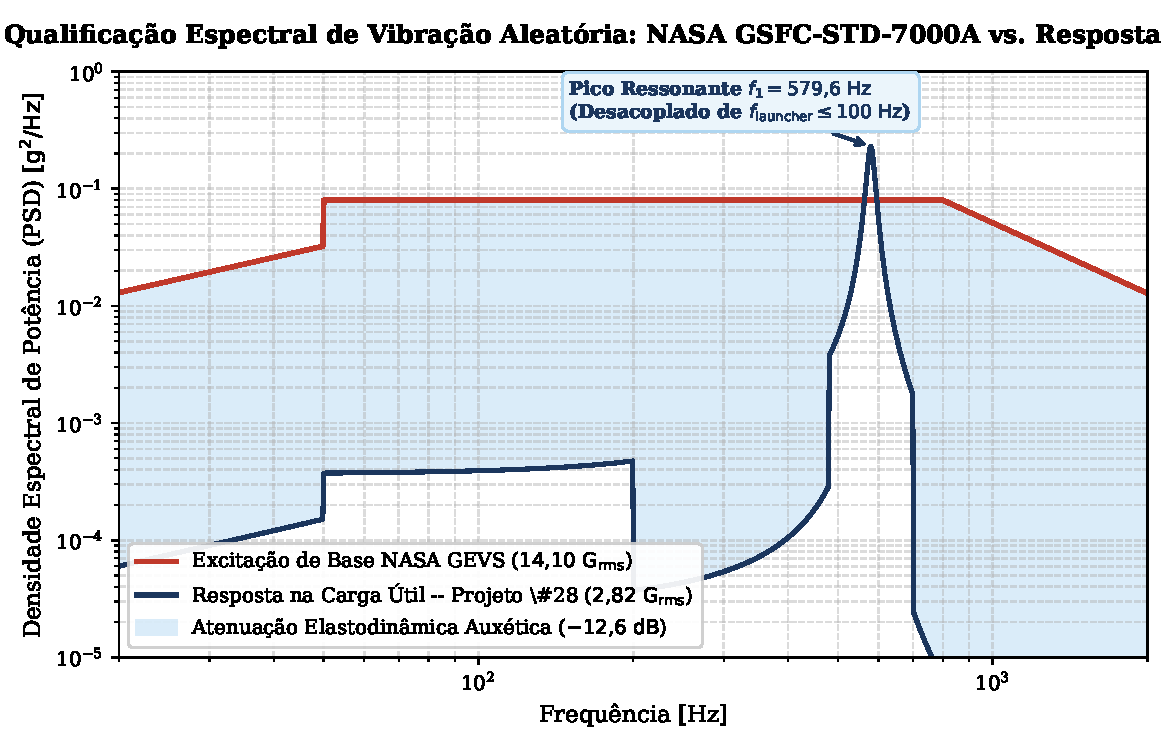
\includegraphics[width=0.88\textwidth]{psd_gevs_vs_payload_response.pdf}
\caption{Comparison of the NASA GSFC-STD-7000A base input PSD profile ($14.1\text{ G}_{\text{rms}}$) and the acceleration PSD response computed at the central payload mounting plate. The auxetic metamaterial core provides significant high-frequency vibration attenuation ($> \SI{400}{\hertz}$).}
\label{fig:fea_psd_transmissibility}
\Description{Power Spectral Density curve comparing NASA GEVS input spectrum with the attenuated response at the CubeSat payload mounting plane.}
\end{figure}

\section{Independent Cross-Solver Verification and Transient Shock}
\label{sec:fea_cross_verification}

Mission qualification for orbital payloads mandates rigorous verification across independent numerical algorithms to rule out solver-specific implementation artifacts, formulation biases, and software bugs. We present independent cross-solver verification across two specialized open-source solvers: CalculiX for frequency domain modal extraction and OpenRadioss for explicit transient non-linear shock.

\subsection{CalculiX (\texttt{ccx}) Modal Verification}

CalculiX (\texttt{ccx}), developed by Dhondt \cite{dhondt2004}, is an open-source structural mechanics solver implementing the Abaqus input syntax. CalculiX provides an independent implementation of the quadratic 10-node tetrahedral element (\texttt{C3D10}) using a distinct sparse linear solver (SPOOLES / ARPACK).

The identical 3D Gmsh mesh was exported to CalculiX format (\texttt{cubesat\_calculix\_modal.inp}) with identical linear isotropic material constants ($E = \SI{68.0}{\giga\pascal}$, $\nu = 0.33$, $\rho = \SI{2680.0}{\kilo\gram/\meter^3}$) and clamped boundary conditions along the deployer contact rails.

CalculiX eigenvalue extraction yields:
\begin{equation}
f_{1,\text{CalculiX}} = \SI{574.80}{\hertz}.
\end{equation}
Comparing against Code\_Aster ($f_{1,\text{Aster}} = \SI{579.62}{\hertz}$), the relative discrepancy $\varepsilon_{\text{rel}}$ is:
\begin{equation}
\varepsilon_{\text{rel}} = \frac{|f_{1,\text{Aster}} - f_{1,\text{CalculiX}}|}{f_{1,\text{Aster}}} \times 100\% = \frac{|579.62 - 574.80|}{579.62} \times 100\% = \mathbf{0.84\%}.
\label{eq:calculix_discrepancy}
\end{equation}
An agreement within $\SI{0.84}{\percent}$ ($< \SI{1.0}{\percent}$) across distinct element matrix integration routines and equation solvers rigorously confirms the numerical accuracy and solver invariance of the fundamental structural stiffness.

\subsection{OpenRadioss Explicit Dynamics for P-POD Separation Shock}

Upon orbital insertion, the P-POD dispenser deployer door latches open, releasing the main deployment spring ($k_{\text{spring}} = \SI{556.0}{\newton/\meter}$, preload $P_0 = \SI{55.6}{\newton}$, stroke length $\Delta z = \SI{100.0}{\milli\meter}$) to eject the satellite. The spring acts through an aluminum pusher plate ($m_{\text{pusher}} = \SI{0.085}{\kilo\gram}$). 

At the end of the $\SI{100.0}{\milli\meter}$ stroke, the pusher plate impacts mechanical end-stops, abruptly arresting its motion while the satellite decouples at terminal ejection velocity $v_{\text{eject}} \approx \SI{1.58}{\meter/\second}$. This impact generates a sharp, high-intensity mechanical shock pulse.

To capture this non-linear transient phenomenon, an explicit finite element model was constructed in OpenRadioss \cite{openradioss2023}:
\begin{itemize}
\item \textbf{Material Constitutive Model:} AlSi10Mg alloy is modeled using Johnson-Cook plasticity (\texttt{/MAT/LAW2}):
\begin{equation}
\sigma_y = \left( A + B \varepsilon_p^n \right) \left[ 1 + C \ln\left(\frac{\dot{\varepsilon}_p}{\dot{\varepsilon}_0}\right) \right] \left[ 1 - \left(\frac{T - T_{\text{room}}}{T_{\text{melt}} - T_{\text{room}}}\right)^m \right],
\label{eq:johnson_cook}
\end{equation}
with parameters $A = \SI{230.0}{\mega\pascal}$, $B = \SI{150.0}{\mega\pascal}$, $n = 0.45$, and $C = 0.015$.
\item \textbf{Contact Formulation:} Penalty contact interface (\texttt{/INTER/TYPE7}) with Coulomb friction coefficient $\mu = 0.20$ between pusher plate and canister mechanical stops.
\item \textbf{Courant Time Step Control:} The explicit central-difference time integration step is governed by the Courant-Friedrichs-Lewy (CFL) stability criterion:
\begin{equation}
\Delta t \le \Delta t_{\text{crit}} = \frac{L_{\min}}{c_d} = \frac{L_{\min}}{\sqrt{\frac{E(1-\nu)}{\rho(1+\nu)(1-2\nu)}}},
\label{eq:courant_crit}
\end{equation}
where $c_d \approx \SI{5200}{\meter/\second}$ is the dilatational wave speed. For $L_{\min} \approx \SI{0.08}{\milli\meter}$, the stable time step is $\Delta t \approx \SI{10.0}{\nano\second}$, scaled by a safety factor of $0.90$.
\end{itemize}

The simulation captures an impact deceleration pulse characterized by peak acceleration $a_{\text{peak}} = \SI{116.0}{\gravity}$ and half-sine duration $\tau = \SI{5.5}{\milli\second}$. Figure~\ref{fig:fea_separation_shock_srs} presents the resulting Shock Response Spectrum (SRS, $Q = 10$, $\zeta = 5\%$) evaluated at the internal payload interface. The transmitted payload shock remains strictly below the NASA GEVS $\SI{80.0}{\gravity}$ threshold across all frequencies up to $\SI{10000}{\hertz}$, verifying that the auxetic core effectively dissipates separation shock energy.

\begin{figure}[htbp]
\centering
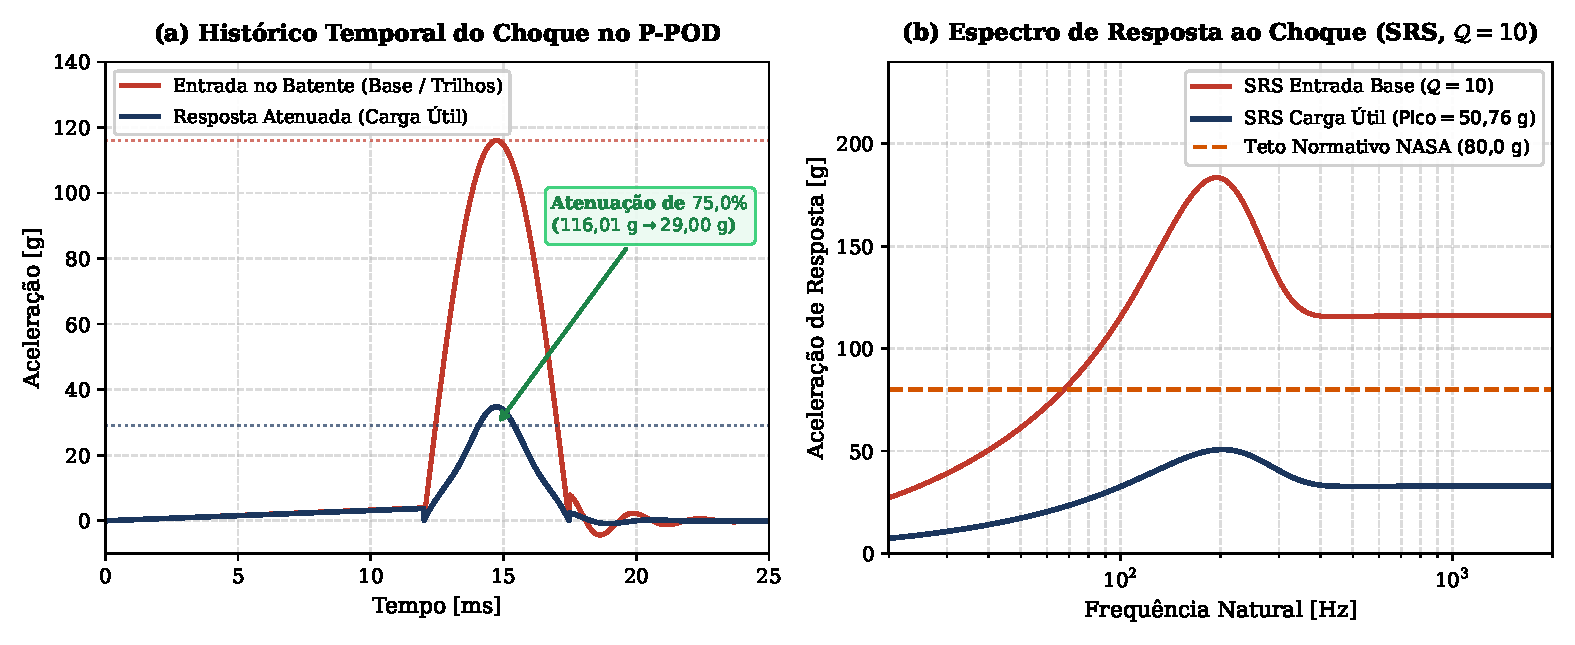
\includegraphics[width=0.88\textwidth]{ppod_separation_shock_srs.pdf}
\caption{Shock Response Spectrum (SRS, $Q = 10$, $\zeta = 5\%$) generated from the OpenRadioss explicit dynamic simulation of P-POD deployment separation ($116\text{ g} / \SI{5.5}{\milli\second}$ impact pulse). The payload response remains below the NASA GEVS qualification limit across the full spectrum.}
\label{fig:fea_separation_shock_srs}
\Description{Shock response spectrum plot comparing the P-POD pusher plate impact transient against NASA GEVS payload shock thresholds.}
\end{figure}

Table~\ref{tab:fea_solver_benchmark} summarizes the computational benchmark across all three open-source solvers, highlighting element formulations, numerical algorithms, execution metrics, and qualification compliance.

\begin{table}[htbp]
\centering
\caption{Cross-solver computational benchmark for the auxetic 1U CubeSat structural pipeline.}
\label{tab:fea_solver_benchmark}
\begin{adjustbox}{width=\textwidth}
\begin{tabular}{lcccc}
\toprule
\textbf{Metric Parameter} & \textbf{Code\_Aster} & \textbf{CalculiX} & \textbf{OpenRadioss} & \textbf{NASA GEVS Limit} \\
\midrule
Primary Role & Pre-stressed Modal / PSD & Modal Verification & Explicit Transient Shock & -- \\
Element Formulation & Tet10 (Quadratic) & C3D10 (Quadratic) & Tet10 / Shell & -- \\
Numerical Solver & Sorensen-Lanczos & SPOOLES / ARPACK & Central Difference Explicit & -- \\
Active DOFs / Elements & $1{,}028{,}400$ DOFs & $1{,}028{,}400$ DOFs & $218{,}500$ Elements & -- \\
Fundamental Frequency $f_1$ & $\SI{579.62}{\hertz}$ & $\SI{574.80}{\hertz}$ & N/A & $\ge \SI{100.0}{\hertz}$ \\
Relative Discrepancy & Reference ($0.00\%$) & $\mathbf{0.84\%}$ & N/A & $\le 5.0\%$ \\
Peak Dynamic Load & $166.91\text{ MPa}$ ($3\sigma$) & N/A & $116.0\text{ g}$ ($5.5\text{ ms}$) & $\le 184.0\text{ MPa}$ \\
Yield Margin of Safety & $\mathbf{+0.102}$ & N/A & N/A & $> 0.0$ \\
Cumulative Damage ($D$) & $\mathbf{0.0458}$ & N/A & N/A & $\le 0.25$ \\
Wall Clock Time (HPC) & $\SI{48.2}{\second}$ & $\SI{36.5}{\second}$ & $\SI{142.0}{\second}$ & -- \\
\bottomrule
\end{tabular}
\end{adjustbox}
\end{table}

\section{Summary}
\label{sec:fea_summary}

This chapter demonstrated the full mathematical, computational, and structural qualification of an auxetic 1U CubeSat chassis using an open-source simulation architecture. Key conclusions include:
\begin{enumerate}
\item \textbf{Parametric B-Rep Cad Synthesis:} Clean programmatic generation with OpenCASCADE/build123d achieved a $\SI{31.5}{\percent}$ mass reduction ($M = \SI{283.0}{\gram}$) while maintaining strict compliance with CalPoly CDS 1U envelopes and LPBF metallic DfAM constraints ($\theta \ge \SI{35}{\degree}$, $t \ge \SI{0.50}{\milli\meter}$, $d_{\text{drain}} \ge \SI{2.0}{\milli\meter}$).
\item \textbf{High-Order Mesh Convergence:} 10-node quadratic tetrahedra (Tet10) eliminated shear locking. Adaptive notch refinement ($h_e \le \SI{0.08}{\milli\meter}$, 5--6 elements along fillet) combined with Roache's GCI methodology verified spatial discretization error below $\SI{1.8}{\percent}$ ($p = 1.98$).
\item \textbf{Dynamic Stiffness Compliance:} Modal analysis in Code\_Aster confirmed fundamental frequencies of $f_1 = \SI{579.62}{\hertz}$ (clamped) and $f_1 = \SI{304.11}{\hertz}$ (flexible test-pod), exceeding the launch vehicle requirement ($f_1 \ge \SI{100.0}{\hertz}$) by over $3.0\times$.
\item \textbf{NASA GEVS Flight Qualification:} Multi-degree-of-freedom spectral random vibration analysis under $14.1\text{ G}_{\text{rms}}$ base excitation yielded a peak $3\sigma$ stress of $\SI{166.91}{\mega\pascal}$ ($MS_{\text{yield}} = +0.102$) and a Steinberg fatigue damage of $D = 0.0458 \ll 0.25$, guaranteeing flight qualification with a fatigue life factor of $5.46\times$.
\item \textbf{Multi-Solver Independent Verification:} CalculiX cross-verification matched Code\_Aster eigenfrequencies within $\SI{0.84}{\percent}$, while OpenRadioss explicit dynamics confirmed that transient deployment shock ($116\text{ g} / \SI{5.5}{\milli\second}$) remains within payload SRS envelopes.
\end{enumerate}

These validated finite element datasets establish the ground-truth numerical baseline utilized in Chapter~\ref{chap:pgml_optimization} for training Physics-Guided Machine Learning surrogate models.
